% !TEX root = ../my_thesis.tex

\section{Training des Convolutional Neural Networks}
Die Architektur der künstlichen neuronalen Netzen bzw. CNNs werden grundsätzlich zuerst aufgabenspezifisch konstruiert und anschließend die Netze mit entsprechenden Daten trainiert. In der vorliegenden Arbeit wird als Netzwerk das in Abschnitt \ref{sec:posenet} beschriebene PoseNet Modell verwendet. Die Arbeit folgt den Ansatz von \citet{acharyaBIMPoseNetIndoorCamera2019} mit Gradienten- bzw. Kantenbilder der synthetischen Daten das Netzwerk zu trainieren, um anschließend mit Gradientenbilder der realen Daten das Netzwerk zu evaluieren. 


Im weiteren Verlauf dieses Kapitel werden die Datensätze angegeben. Danach wird die Erhebung / Generierung der realen / synthetischen Daten beschrieben und die Verarbeitung der Daten dargestellt. Im Anschluss werden die Trainingsparameter angegeben. 

\subsection{Datensätze}
\label{subsec:datasets}
In dieser Arbeit werden aus zwei unterschiedlichen Gebäuden Daten erhoben bzw. synthetische Daten aus den Gebäudesimulationen generiert. 
Zuerst wird ein Datensatz aus der nördlichen Hälfte des 6. Stockwerkes des IC-Gebäudes Ruhr-Universität Bochum (\textit{IC}) erhoben. Anschließend werden drei Datensätzen im Seminargebäude Hochschule Bochum (\textit{HS}) erhoben. Die Gebäude unterscheiden sich im Detail der Simulationen. Die Simulation vom IC enthält sehr wenige Objekte wie z.B. Türen und Wände. Im Gegensatz dazu enthält die HS Simulation mehr Objekte wie z.B. die Objekte der technischen Gebäudeausrüstung. Abbildung \ref{fig:difference_3d} veranschaulicht die Simulationen.


\begin{figure}[H]
	\centering
	\begin{subfigure}[t]{0.48\linewidth}
		\centering
		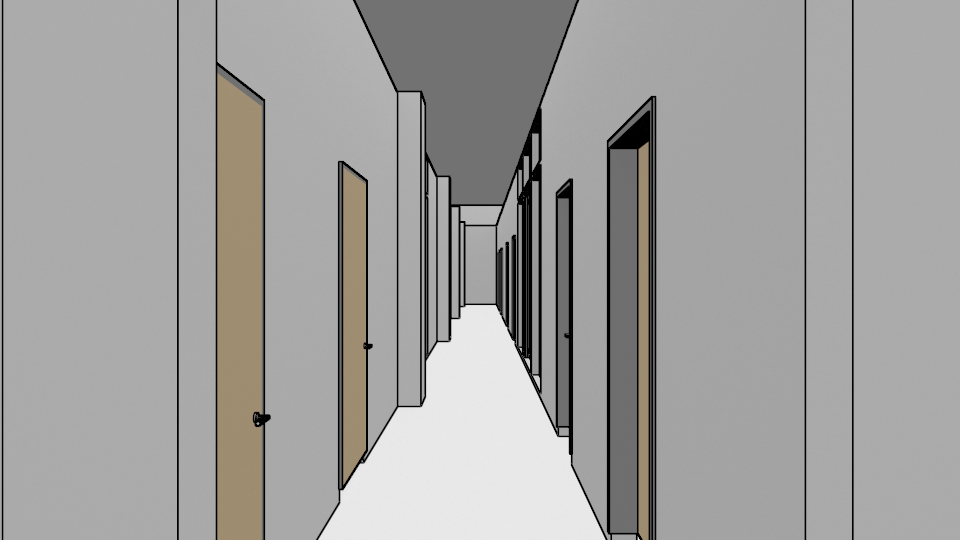
\includegraphics[width=\linewidth]{images/syn_dataset/ic00343.png}
		\caption{IC Simulation}
		\label{subfig:ic_syn_example}
	\end{subfigure}
	\hfill
	\begin{subfigure}[t]{0.48\linewidth}
		\centering
		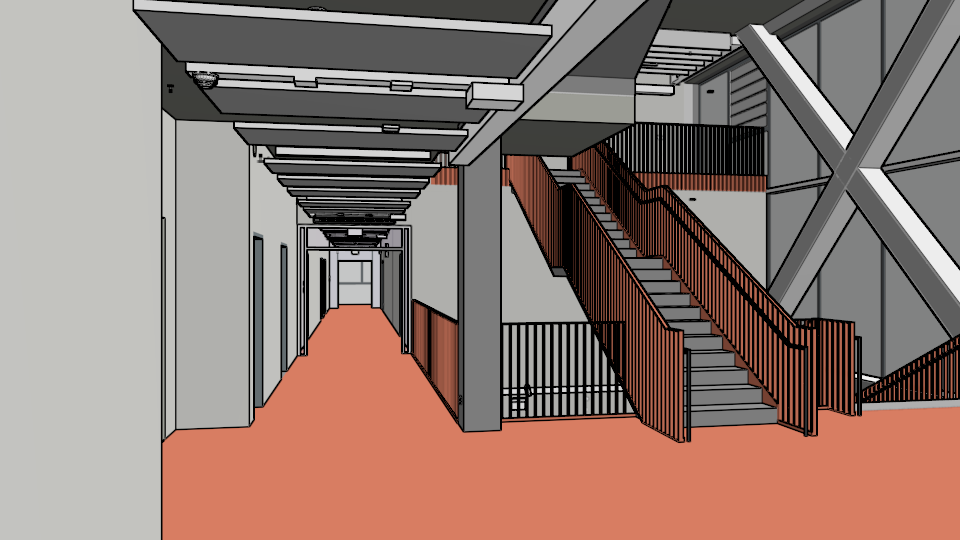
\includegraphics[width=\linewidth]{images/syn_dataset/hs_gamma02162.png}
		\caption{HS Simulation}
		\label{subfig:hs_gamma_syn_example}
	\end{subfigure}
	\caption{Veranschaulichung der Gebäudesimulationen. Die Kanten sind markant dargestellt. Im Vergleich zu \subref{subfig:ic_syn_example} ist die Decke von \subref{subfig:hs_gamma_syn_example} detailreicher. Während die Wände und der Boden in \subref{subfig:ic_syn_example} monoton sind, sind diese in \subref{subfig:hs_gamma_syn_example} mit teschnichen Gebäudeausrüstüngen wie z.B. Steckdose beschmückt.}
	\label{fig:difference_3d}
\end{figure}

Die ca. $115m$ lange Strecke im ersten Datensatz, bezeichnet als \textit{IC-loop}, bildet eine geschlossene Schleife in einem $50m \times 11m \times 3.5m$ Bereich der IC. Die $65m$ lange Strecke im \textit{HS-gamma} Datensatz einhält in der Mitte eine Schleife und übergeht zu einem optisch ähnlichen Flur wie der Ausgangsflur in einem Bereich von ca. $54m \times 10m \times 3m$ der HS. Im Datensatz \textit{HS-stairs-up} wird eine Treppe im HS aufwärts bestiegen und im Datensatz \textit{HS-stairs-down} dieselbe Treppe abgestiegen. Die Strecken auf den Treppen sind ca. $32m$ lang und befindet sich in einer ca. $12m \times 12m \times 12m$ Teilzone von HS.
Alle Datensätze beinhalten Herausforderungen wie z.B. das \textit{Loop-Closure}- oder \textit{Perceptual-Aliasing}-Problem.
Tabelle \ref{tab:dataset_metrics} listet die approximierten metrischen Eigenschaften der Datensätze auf. 

\begin{table}[H]
	\centering
	\caption{Approximierte metrische Eigenschaften der Datensätze.}
	\begin{tabularx}{1.0\textwidth}{X X X >{\centering\arraybackslash}p{1.7cm} }
		\textbf{Bezeichnung} & \textbf{Streckenlänge} & \textbf{Volumen} & \textbf{Gebäude}\\
		\hline
		IC-loop & $115m$ & $50m \times 11m \times 3.5m$ & IC \\
		\hline
		HS-gamma & $65m$ & $54m \times 10m \times 3m$ & HS\\
		\hline
		HS-stairs-up & $32m$ & $12m \times 12m \times 12m$ & HS\\
		\hline
		HS-stairs-down & $32m$ & $12m \times 12m \times 12m$ & HS\\
	\end{tabularx}
	\label{tab:dataset_metrics}
\end{table}




Die Verschiedenheit der Streckenlänge führt logischweiße in den Datensätzen zu unterschiedlicher Anzahl an realen sowie synthetischen Daten. Tabelle \ref{tab:datasets} stellt die Anzahl der Daten in den Datensätzen dar.
Abbildung \ref{fig:trajectories} illustriert die Strecken der synthetischen Datensätze. 


\begin{table}[H]
	\centering
	\caption{Datenanzahl der Datensätze.}
	\begin{tabularx}{1.0\textwidth}{p{3.5cm} p{1.8cm} X  >{\centering\arraybackslash}p{1.7cm} }
		\textbf{Bezeichnung} & \textbf{Typ} & \textbf{Anzahl Daten} & \textbf{Gebäude}\\
		\hline
		IC-loop & real & 3842 & IC\\
		\hline
		IC-loop-syn & synth. & 11435 & IC\\
		\hline
		HS-gamma & real & 1958 & HS\\
		\hline
		HS-gamma-syn & synth. &  6490 & HS\\
		\hline
		HS-stairs-up & real & 1068 & HS\\
		\hline
		HS-stairs-up-syn & synth. & 3160 & HS\\
		\hline
		HS-stairs-down & real & 1161 & HS\\
		\hline
		HS-stairs-down-syn & synth. &  3245 & HS\\
	\end{tabularx}
	\label{tab:datasets}
\end{table}


\cleardoublepage

\begin{figure}[H]
	\centering
	\begin{subfigure}[t]{1.0\linewidth}
		\centering
		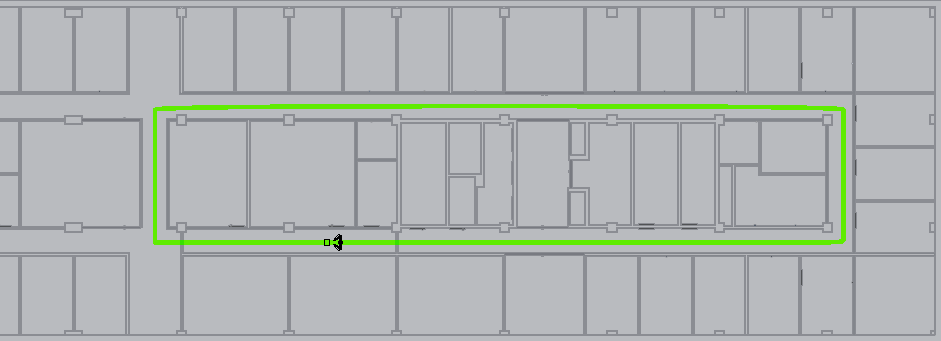
\includegraphics[width=\linewidth]{images/trajectories/traj-ic.png}
		\caption{\textit{IC-loop}}
		\label{subfig:traj_ic}
	\end{subfigure}
	\hfill \medskip
	\begin{subfigure}[t]{1.0\linewidth}
		\centering
		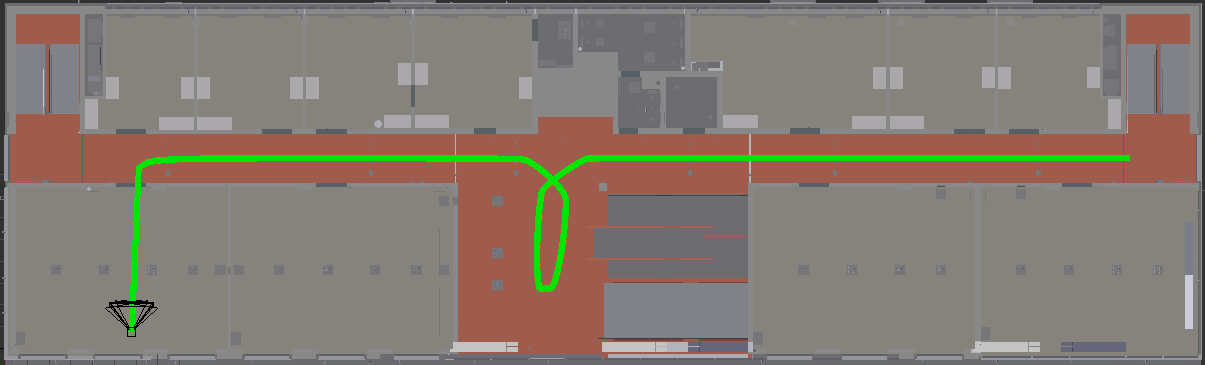
\includegraphics[width=\linewidth]{images/trajectories/traj-hs-gamma.png}
		\caption{\textit{HS-gamma}}
		\label{subfig:traj_hs_gamma}
	\end{subfigure}
	\hfill \medskip
	\begin{subfigure}[tr]{0.45\linewidth}
		\flushleft
		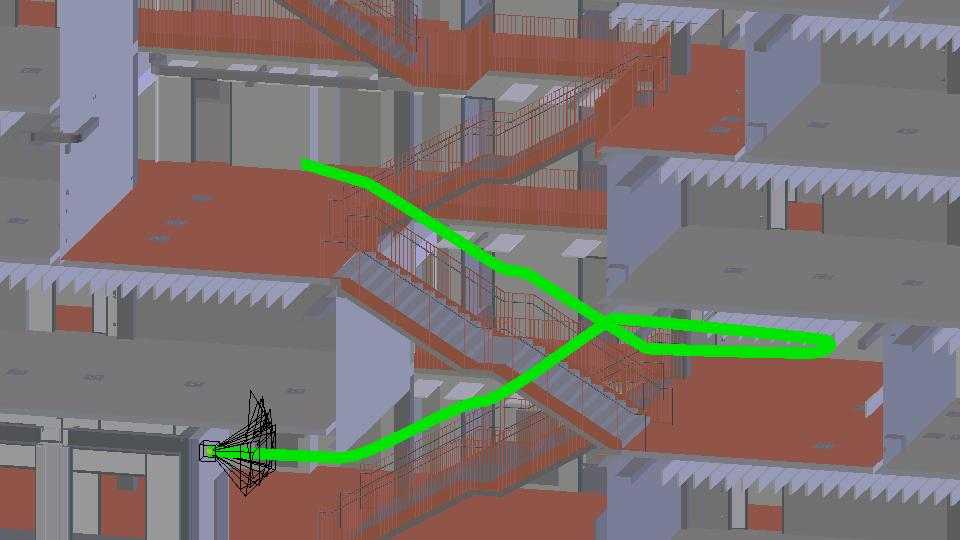
\includegraphics[width=\linewidth]{images/trajectories/traj-stairs-up.png}
		\caption{\textit{HS-stairs-up}}
		\label{subfig:traj_hs-up}
	\end{subfigure}
	\hfill
	\begin{subfigure}[tl]{0.45\linewidth}
		\flushright		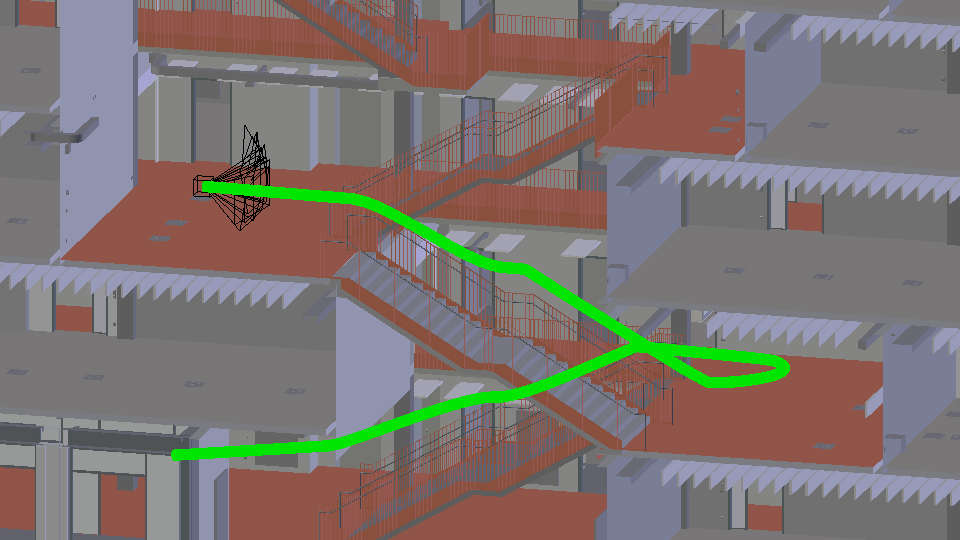
\includegraphics[width=\linewidth]{images/trajectories/traj-stairs-down.png}
		\caption{\textit{HS-stairs-down}}
		\label{subfig:traj_hs-down}
	\end{subfigure}
	\hfill
	\caption{Illustration der Aufnahmestrecken der synthetischen Datensätze. Die Aufnahmestrecken wurden grün im Vordergrund gekennzeichnet. \subref{subfig:traj_ic} befindet sich in der nördlichen Hälfte des 6. Stockwerkes des IC-Gebäudes Ruhr-Universität Bochum. \subref{subfig:traj_hs_gamma}, \subref{subfig:traj_hs-up}, \subref{subfig:traj_hs-down} befinden sich im Seminargebäude Hochschule Bochum. \subref{subfig:traj_hs-up} und \subref{subfig:traj_hs-down} sind nahe an der Position der Schleife von \subref{subfig:traj_hs_gamma}. Tabelle \ref{tab:dataset_metrics} listet die approximierten metrischen Eigenschaften der Aufnahmestrecken auf.}
	\label{fig:trajectories}
\end{figure}


\subsection{Erhebung der realen Daten}
\label{subsec:record_real_data}
In der Literatur wurden die realen Daten einer Zone grundsätzlich entlang einer Strecke aufgenommen \cite{kendallPoseNetConvolutionalNetwork2015, clarkVidLocDeepSpatioTemporal2017, acharyaBIMPoseNetIndoorCamera2019}. Daher werden zuerst die Aufnahmestrecken in den Gebäudesimulationen festgelegt und anschließend die Aufnahmen durchgeführt. Davor werden die Ausgangspunkte der Aufnahmen zu einem Referenzpunkt in den Simulationen abgemessen und als Offset der globalen Position zu den Ground-Truth-Daten addiert.

In der Literatur wurden SfM-Methoden eingesetzt, um die Ground-Truth-Daten der realen Aufnahmen zu bestimmen \cite{kendallPoseNetConvolutionalNetwork2015, clarkVidLocDeepSpatioTemporal2017, acharyaBIMPoseNetIndoorCamera2019}. 
In der vorliegenden Arbeit wird für die Bestimmung der Ground-Truth-Daten sowie die Aufnahme der Bilder zeitgleich zwei unterschiedliche Kameras der Intel Realsense Reihe verwendet. Eine Intel Realsense T265\footnote{\url{https://www.intelrealsense.com/tracking-camera-t265/} (abgerufen am: 18.07.2019)} wird eingesetzt, die die Odometrie (Ground-Truth-Daten) mit einer Abweichung von 1\%  über die SfM von zwei Fischaugenkameras (Auflösung von $848 \times 800$ ) und Inertial Measurement Units (\textit{IMU}) zu ermitteln verspricht. Zudem wird eine Intel Realsense D435\footnote{ \url{https://www.intelrealsense.com/depth-camera-d435/} (abgerufen am: 18.07.2019)} eingesetzt, die eine 3D Punktwolke, ein $1280\times720$ Tiefenbild sowie ein $1920\times1080$ RGB-Bild einer Szene liefert. Die T265 wird über die D435 Kamera montiert (siehe Abbildung \ref{fig:t265_d435}).

\begin{figure}[H]
	\centering
	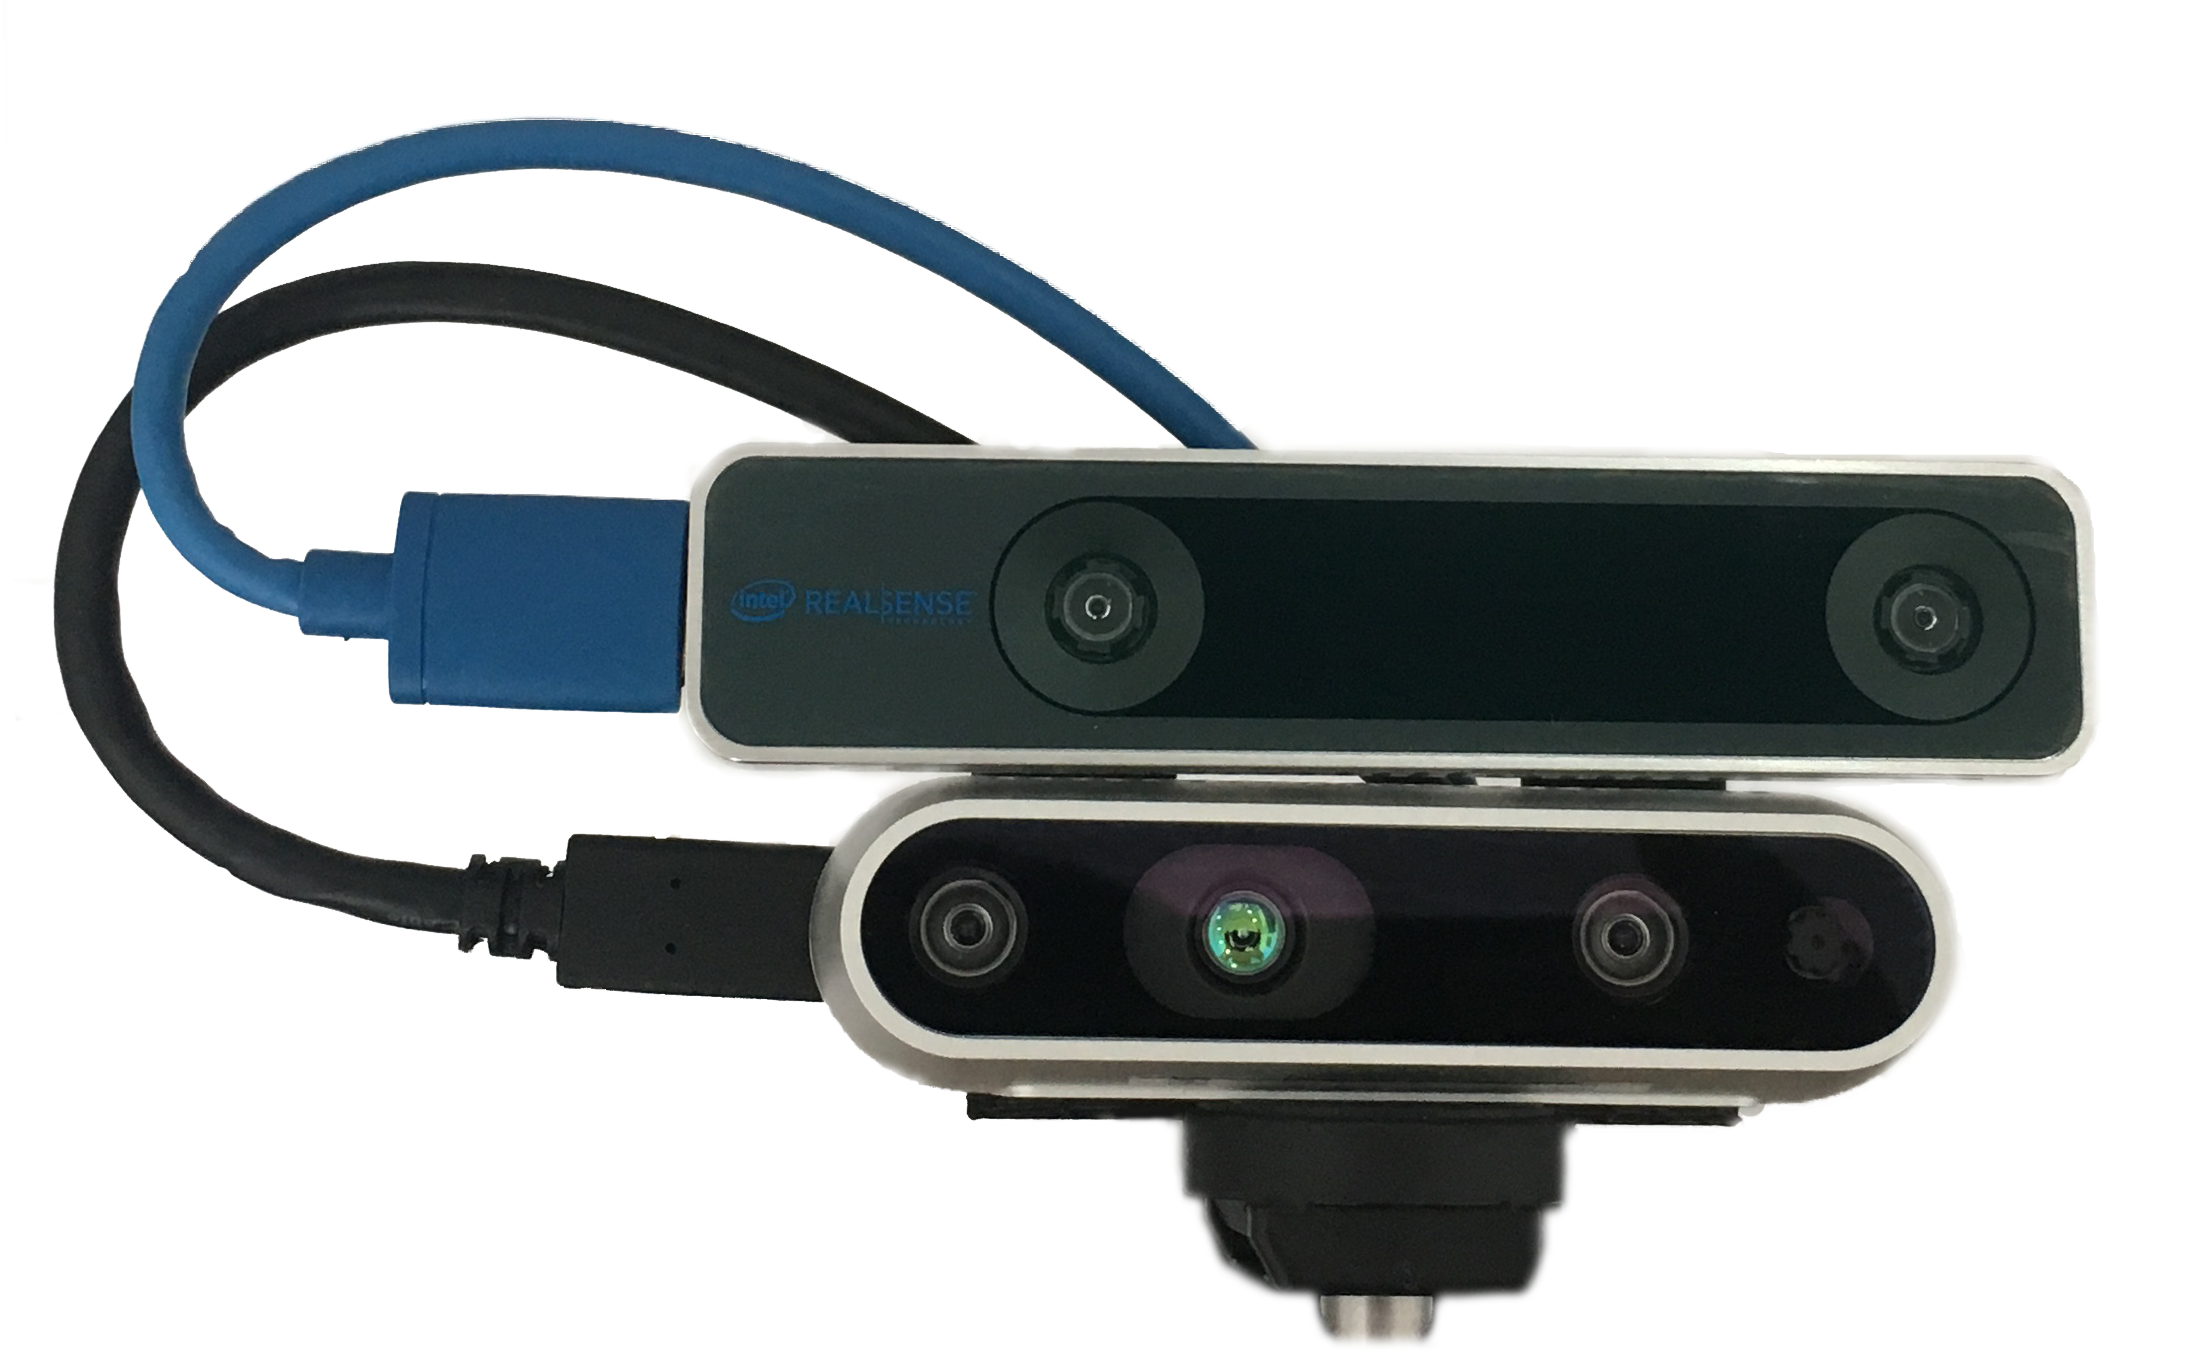
\includegraphics[width=0.5\textwidth]{images/real_dataset/t265_d435_2.png}
	\caption{Hardware für die Aufnahme der realen Daten. Die Intel Realsense T265 ist oberhalb der Intel Realsense D435 montiert. Das Konstrukt kann auf einer universalen Stativschraube befestigt werden.  }
	\label{fig:t265_d435}
\end{figure}

Über das Robot Operating System\footnote{\url{https://www.ros.org/about-ros/} (abgerufen am: 18.07.2019)} (\textit{ROS}) Framework werden die Kameras zeitgleich angesprochen und der Datenfluss der Kameras synchronisiert. Somit beinhaltet jeder Datensatz ein Bild je Fischaugenkamera, ein Tiefenbild, ein RGB-Bild, eine 3D Punktwolke und die dazugehörige Odometrie pro Frame. Für die vorliegende Arbeit sind nur die Odometrie-Daten der T265 sowie die RGB-Bilder der D435 relevant. Abbildung \ref{fig:dataset} visualisiert ein Datensatzexemplar für einen Frame.

\begin{figure}[H]
	\centering
	\begin{subfigure}[t]{0.3\linewidth}
		\centering
		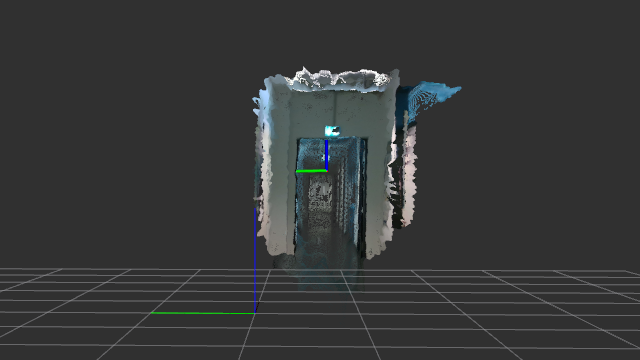
\includegraphics[width=\linewidth]{images/real_dataset/pointcloud3.png}
		\caption{Odometrie  (T265) + \\ 3D Punktwolke (D435)}
		\label{subfig:odom1}
	\end{subfigure}
	\hfill
	\begin{subfigure}[t]{0.3\linewidth}
		\centering
		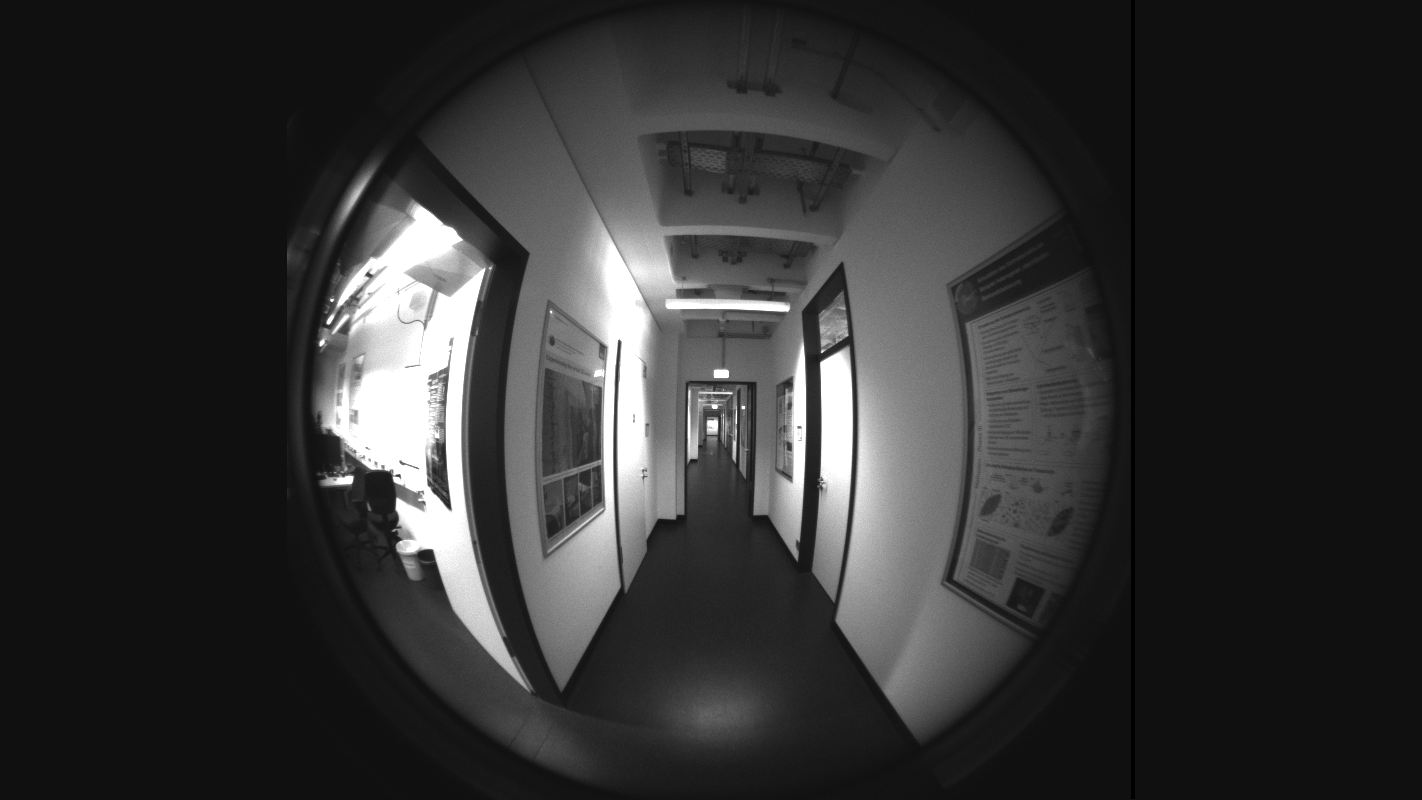
\includegraphics[width=\linewidth]{images/real_dataset/f1_frame000005.png}
		\caption{Fischaugenkamera 1 \\ (T265)}
		\label{subfig:fisheye1}
	\end{subfigure}
	\hfill
	\begin{subfigure}[t]{0.3\linewidth}
		\centering
		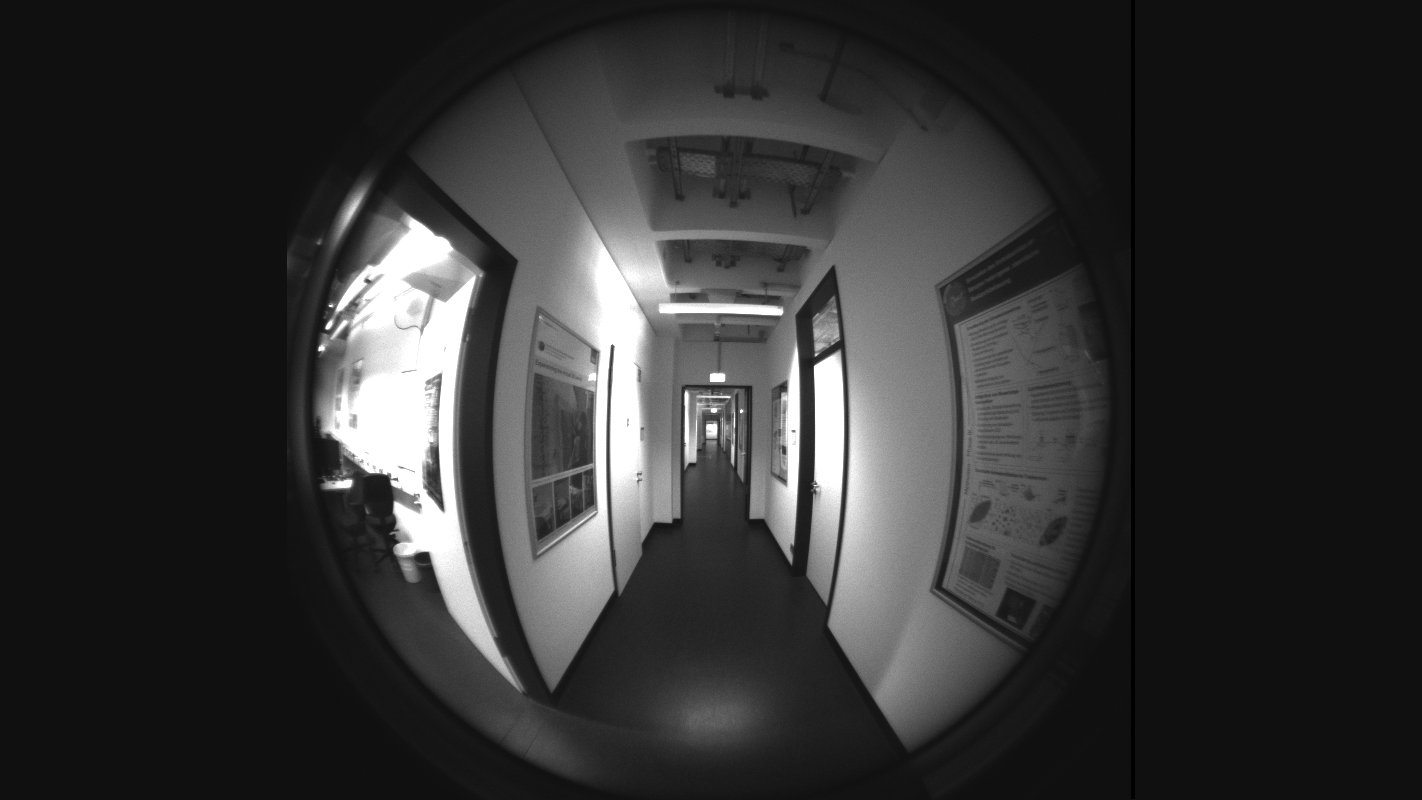
\includegraphics[width=\linewidth]{images/real_dataset/f2_frame000005.png}
		\caption{Fischaugenkamera 2 \\ (T265)}
		\label{subfig:fisheye2}
	\end{subfigure}
	\hfill \medskip
	\begin{subfigure}[t]{0.3\linewidth}
		\centering
		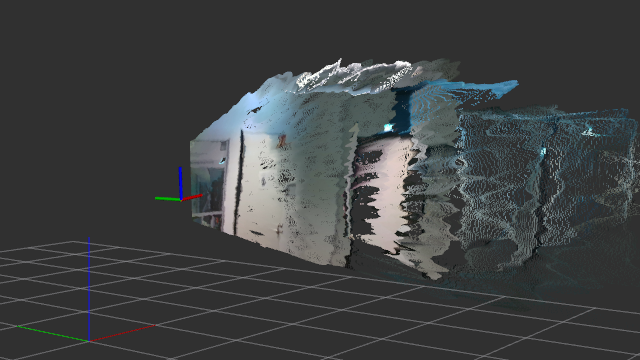
\includegraphics[width=\linewidth]{images/real_dataset/pointcloud1.png}
		\caption{Odometrie  (T265) + \\ 3D Punktwolke (D435)}
		\label{subfig:odom2}
	\end{subfigure}
	\hfill
	\begin{subfigure}[t]{0.3\linewidth}
		\centering
		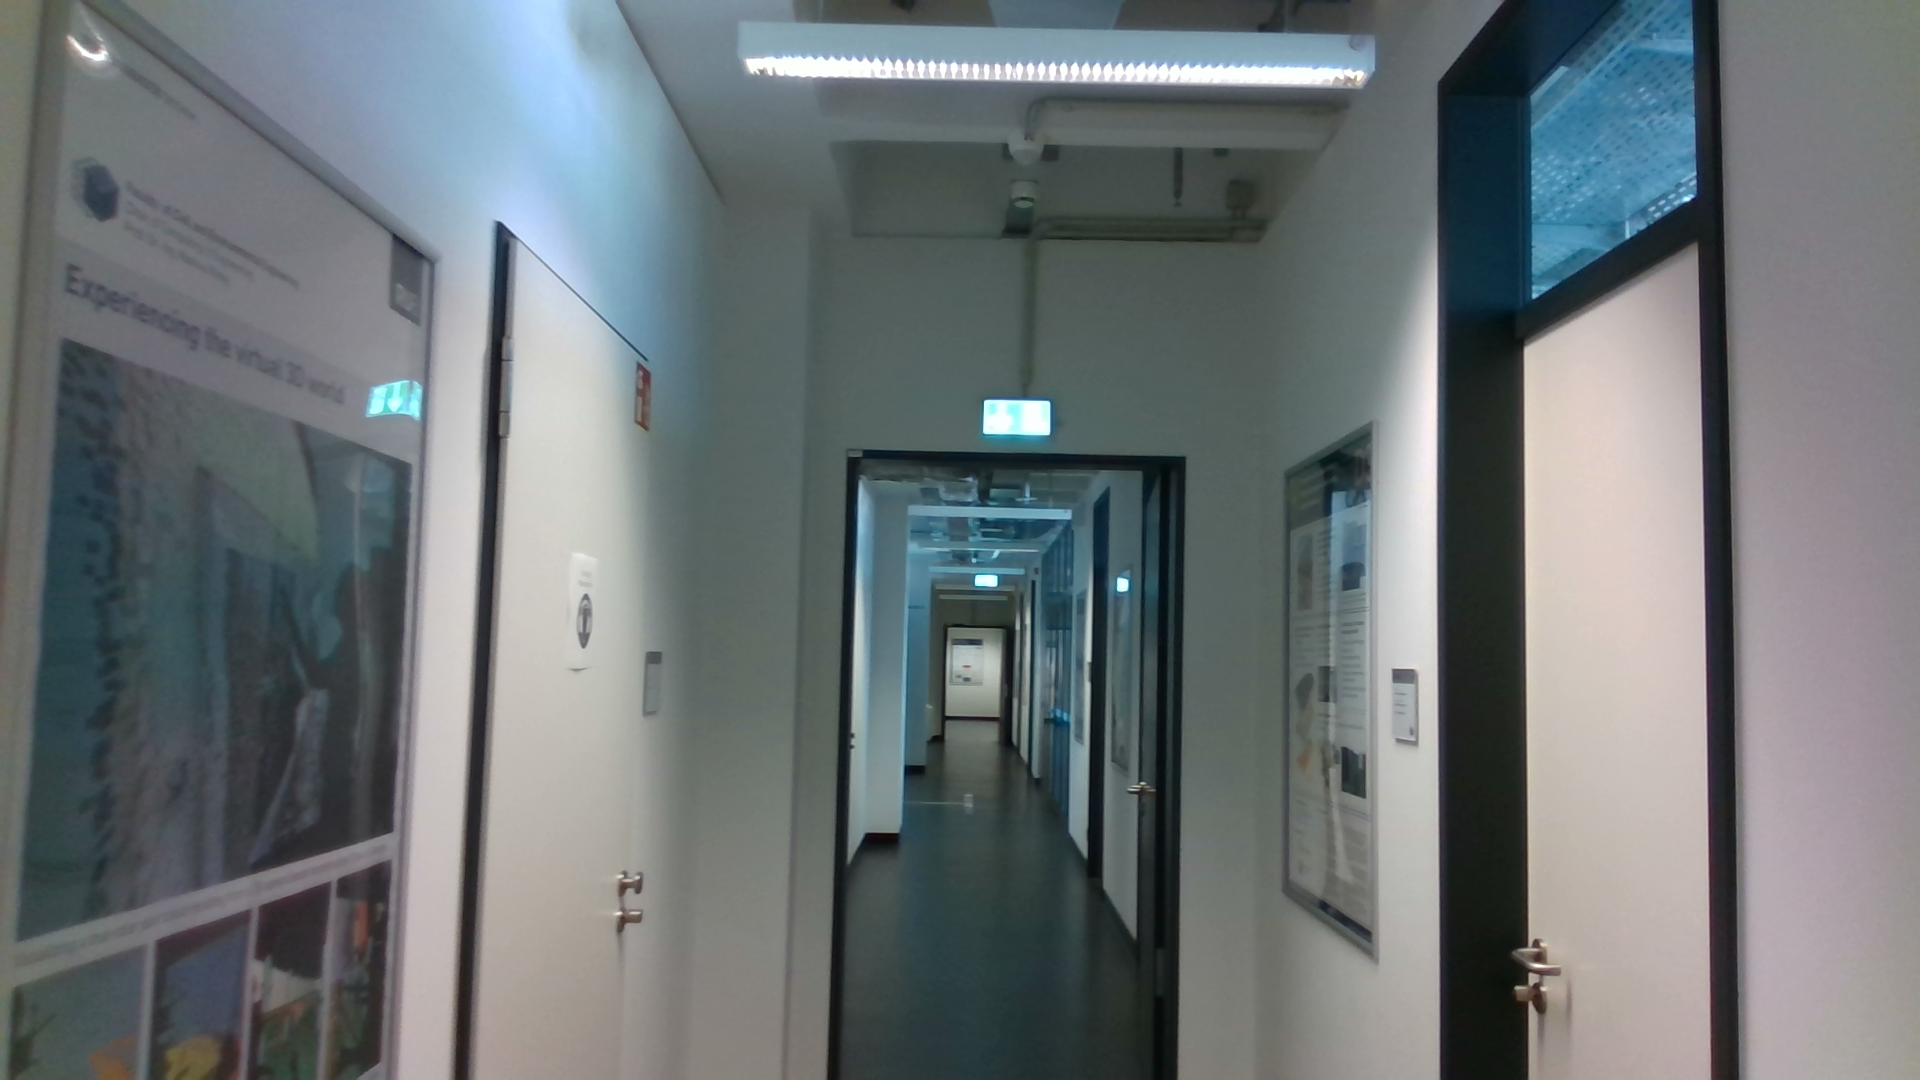
\includegraphics[width=\linewidth]{images/real_dataset/dc_frame000005.png}
		\caption{RGB-Bild \\ (D435) \hspace*{2cm}}
		\label{subfig:rgb-image}
	\end{subfigure}
	\hfill
	\begin{subfigure}[t]{0.3\linewidth}
		\centering
		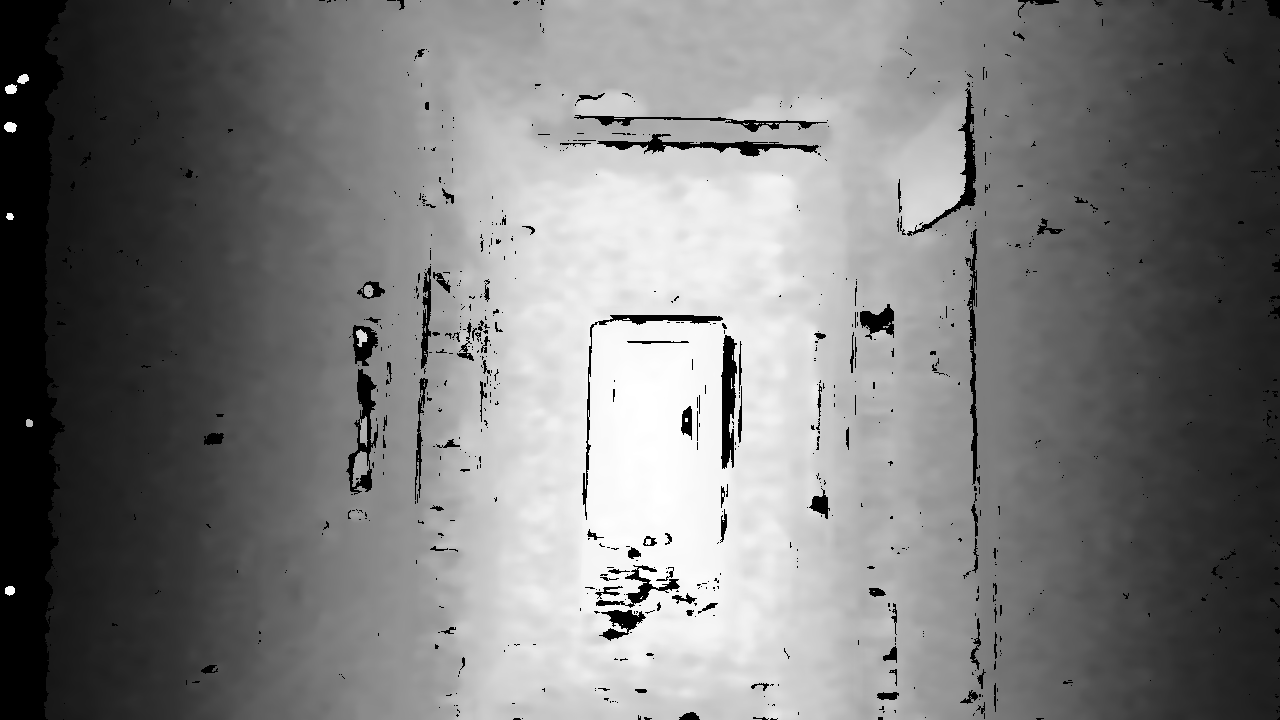
\includegraphics[width=\linewidth]{images/real_dataset/dt_frame000005.png}
		\caption{Tiefenbild \\ (D435) \hspace*{2cm}}
		\label{subfig:depth-image}
	\end{subfigure}
	\caption{Datensatz pro Frame. \subref{subfig:odom1}  und \subref{subfig:odom2} visualisieren in unterschiedlichen Prespektiven die von der T265 ermittelte Odometrie und die von der D435 erhaltenen 3D Punktwolke. \subref{subfig:fisheye1} und \subref{subfig:fisheye2} sind die von der T265 aufgenommenen Fischaugenbilder. \subref{subfig:rgb-image} ist das RGB-Bild der D435 und \subref{subfig:depth-image} das dazugehörige Tiefenbild. }
	\label{fig:dataset}
\end{figure}

\subsection{Generierung der synthetischen Daten}
\label{subsec:generate_synth_images}
Für die Generierung der synthetischen Daten werden aus dem BIM der Gebäuden IC und HS die 3D Modelle entnommen. Die 3D Gebäudemodelle werden in Blender\footnote{\url{https://www.blender.org/about/} (aufgerufen am: 20.07.2019)} Version 2.79b simuliert. Die intrinsischen Daten der D435 RGB-Kamera werden auf die virtuellen Kameras übertragen und aus Zeitgründen wird die Auflösung der synthetischen Bilder auf  $960\times540$ halbiert.

Die Strecken der echten Aufnahmen werden in den Simulationen schwankungslos auf einer konstanten Höhe von 1.70$m$ imitiert.% Die Imitation der Strecke ist nur soweit möglich, wie die Ground-Truth-Daten nicht abdriften. 
Es wird entlang der Strecke in 0.05$m$ Intervallen und mit einer $\pm$10° Neigung in je y- und z-Achse Bilder mit korrespondierenden Ground-Truth-Daten aufgenommen, um die Varianz der realen Daten abzudecken. Abbildung \ref{fig:dataset_variation} illustriert die Variationen der Pose pro Stützpunkt auf einer Strecke.


\begin{figure}[H]
	\centering
	\begin{subfigure}[t]{0.18\linewidth}
		\centering
		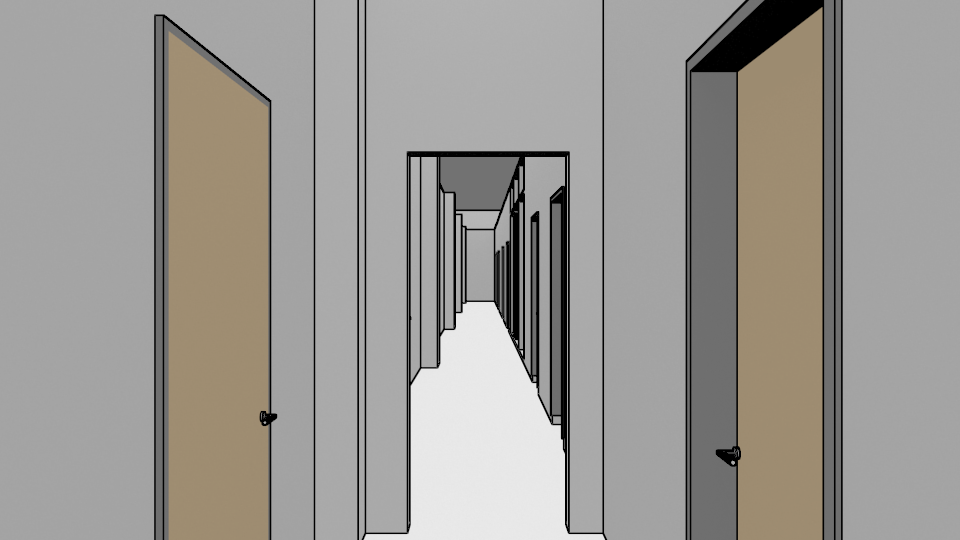
\includegraphics[width=\linewidth]{images/syn_dataset/00023.png}
		\caption{Orginal Pose \vspace{\fill}}
		\label{subfig:iz0_y0}
	\end{subfigure}
	\hfill 
	\begin{subfigure}[t]{0.18\linewidth}
		\centering
		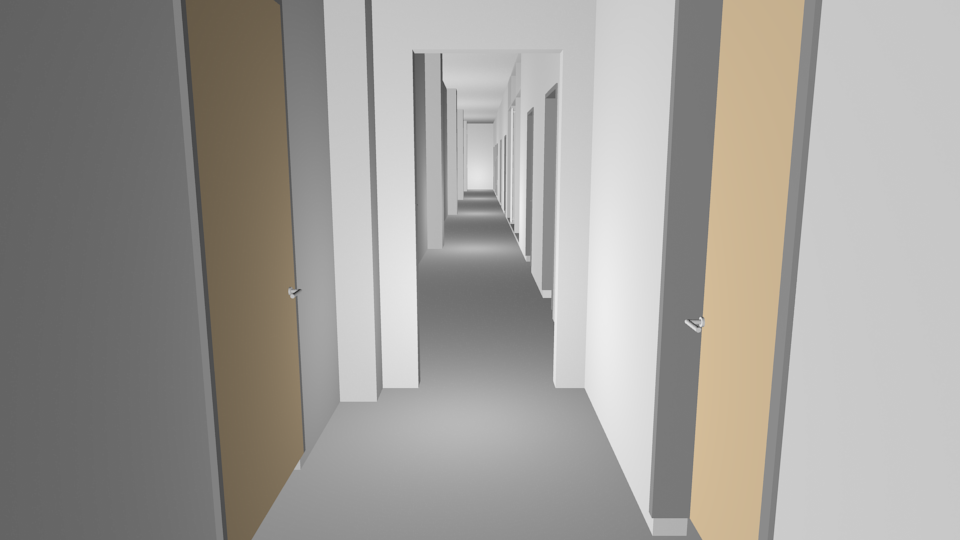
\includegraphics[width=\linewidth]{images/syn_dataset/00021.png}
		\caption{-10° um die y-Achse}
		\label{subfig:iz0_y-10}
	\end{subfigure}
	\hfill
	\begin{subfigure}[t]{0.18\linewidth}
		\centering
		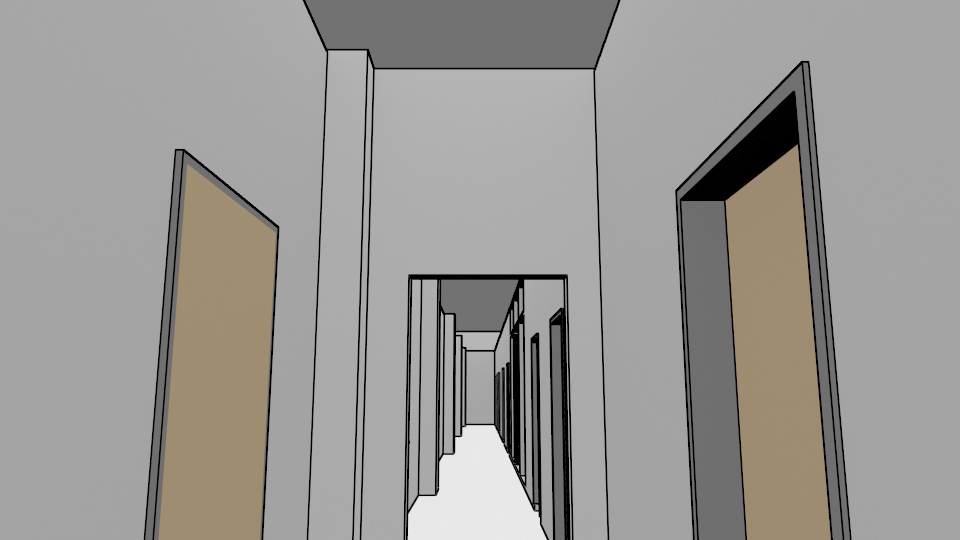
\includegraphics[width=\linewidth]{images/syn_dataset/00020.png}
		\caption{+10° um die y-Achse}
		\label{subfig:iz0_y+10}
	\end{subfigure}
	\hfill
	\begin{subfigure}[t]{0.18\linewidth}
		\centering
		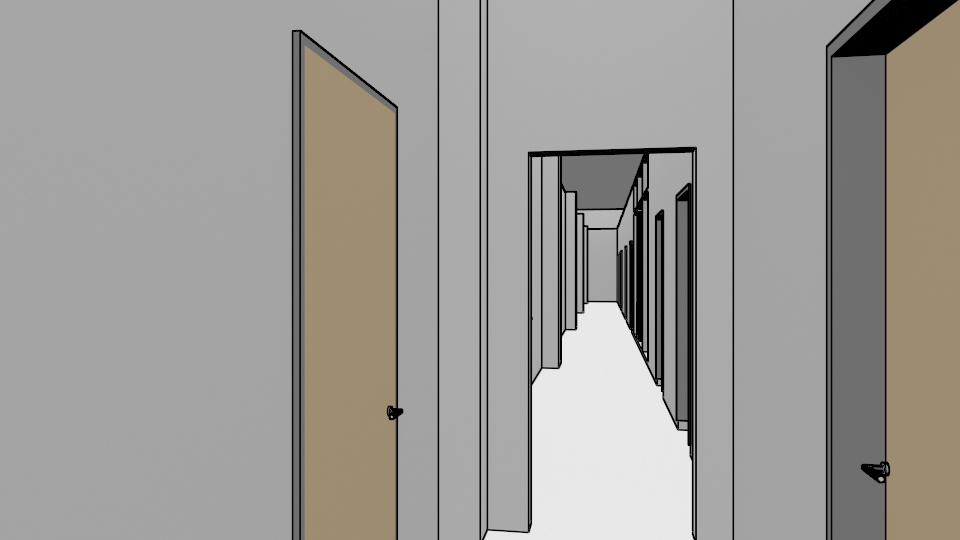
\includegraphics[width=\linewidth]{images/syn_dataset/00024.png}
		\caption{-10° um die z-Achse}
		\label{subfig:iz-10_y0}
	\end{subfigure}
	\hfill
	\begin{subfigure}[t]{0.18\linewidth}
		\centering
		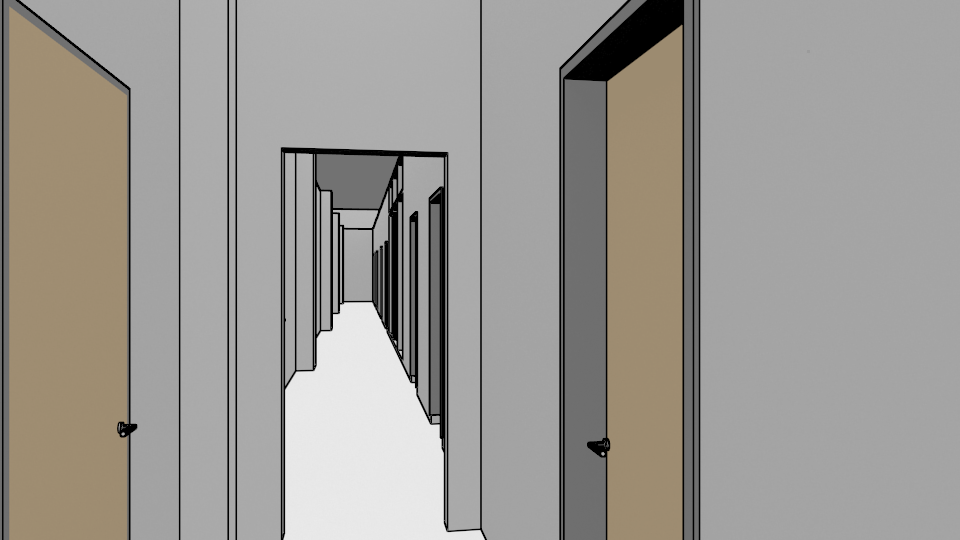
\includegraphics[width=\linewidth]{images/syn_dataset/00022.png}
		\caption{+10° um die z-Achse}
		\label{subfig:iz+10_y0}
	\end{subfigure}
	\caption{Variation der Pose pro Stützpunkt auf einer Strecke.}
	\label{fig:dataset_variation}
\end{figure}

Insgesamt werden drei synthetische Datensätze je Strecke erzeugt, die sich in der Beschaffenheit von karikaturistische Darstellung, zu synthetischen Kantenbilder, hin über zu fotorealistische Darstellung unterscheiden (siehe Abbildung \ref{fig:dataset_preprocess}). Bei der Generierung der karikaturistischen und fotorealistischen Datensätzen wird die Beleuchtung aus einem Netz von Punktlichtquellen nachgestellt.
Für die Erzeugung der synthetischen Kantenbilder wird eine konstante Beleuchtung verschaffen und die Kanten über Blender markant sichtbar konfiguriert. Der karikaturistische Datensatz sowie die Kantenbilder werden über die Render-Engine \textit{Blender Render} und der fotorealistischer Datensatz über die \textit{Cycles-Engine} generiert. Die karikaturistische und fotorealistische Datensätze unterscheiden sich ausschließlich in den Render-Engines.

\subsection{Verarbeitung der Daten}
In der vorliegenden Arbeit wird PoseNet grundsätzlich mit Gradientenbilder trainiert und evaluiert. Bei der Erzeugung von Gradienten- bzw. Kantenbilder gehen einerseits Informationen wie z.B. Texturen vom Ursprungsbild verloren, anderseits bleiben wichtige Informationen wie z.B. die geometrische Strukturen erhalten. Daher sollte ein neuronales Netz beim erfolgreichem Training mit Gradienten- bzw. Kantenbildern sensibler zur geometrische Strukturen und invariant gegenüber Texturen werden.
 
Nach der Erhebung der realen Bilder (siehe Abschnitt \ref{subsec:record_real_data}) und Generierung der synthetischen Bilder (siehe Abschnitt \ref{subsec:generate_synth_images}) werden diese in ihre Gradientenbilder verarbeitet. Die realen Bilder werden vor der Verarbeitung in Gradientenbilder auf die Größe $960 \times 540$ der synthetischen Bilder verkleinert.

Die künstliche Beleuchtung in den Gebäudesimulationen führt bei den Gradientenbildern zu unerwünschten Artefakten (vgl. Abbildung \ref
{fig:treshhold}). Für die Unterdrückung der Artefakten wird zusätzlich ein Schwellenwertverfahren angewendet, indem Pixeln eines Gradientenbildes einen Mindestwert erhalten. Es wird iterativ nach einem Wert gesucht, der die Artefakte in den Gradientenbildern unterdrückt. Der Wert x wird als geeigneter Schwelle definiert. Abbildung \ref{fig:dataset_preprocess} visualisiert von jedem Datensatztyp ein Beispiel und die dazugehörigen Gradientenbilder.


\begin{figure}[H]
	\centering
	\begin{tikzpicture}[zoomboxarray, 
	connect zoomboxes,
	zoomboxarray columns=2,
	zoomboxarray rows=1]
	\node [image node] { \includegraphics[width=0.45\textwidth]{images/treshold/0_treshold.png} };
	\zoombox[magnification=30]{0.15,0.8}
	\zoombox[magnification=30]{0.5,0.25}
	\end{tikzpicture}
	\caption{The National Gallery of Canada}
\end{figure}


\vspace{1cm}
\begin{figure}[H]
	\centering
	\begin{subfigure}[t]{0.24\linewidth}
		\centering
		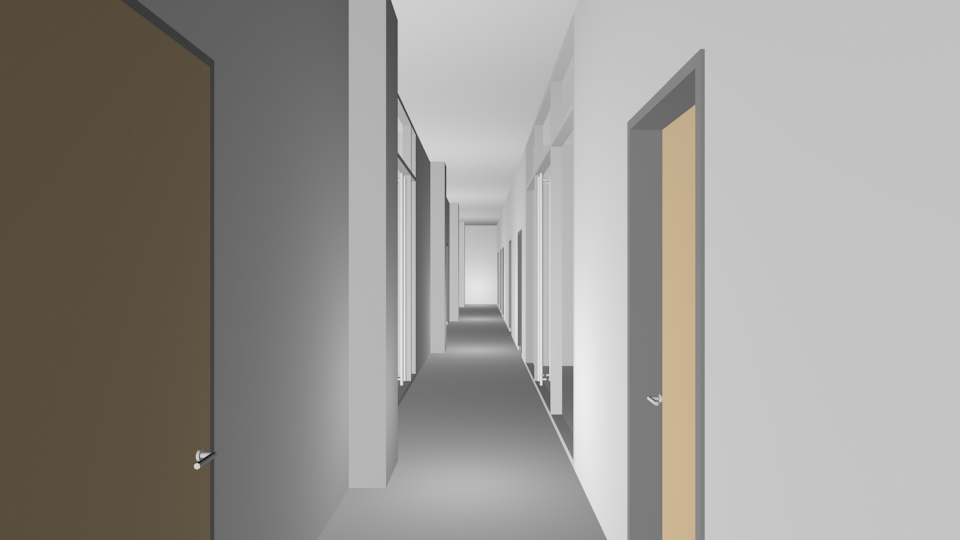
\includegraphics[width=\linewidth]{images/syn_dataset/b00708.png}
		\caption{karikaturistische Simulation}
		\label{subfig:cartoonish}
	\end{subfigure}
	\hfill
	\begin{subfigure}[t]{0.24\linewidth}
		\centering
		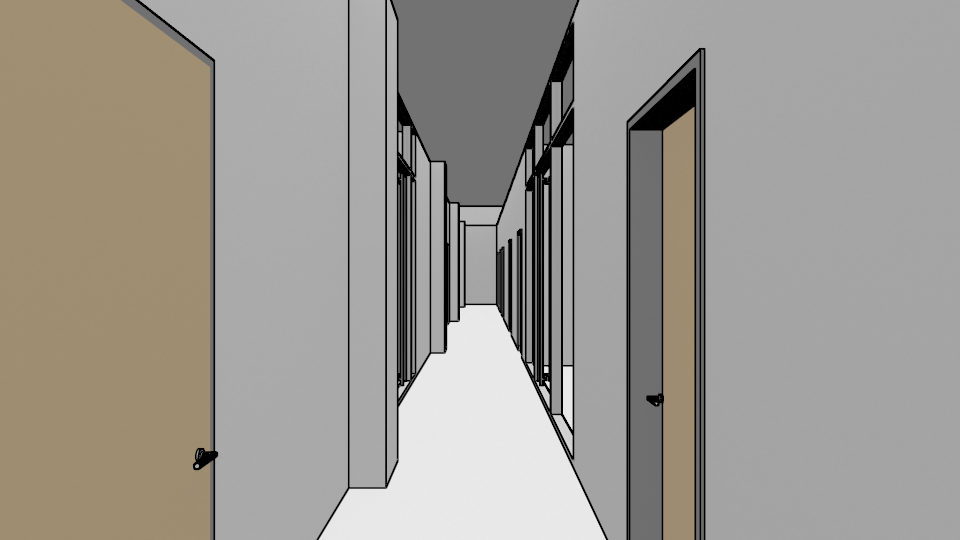
\includegraphics[width=\linewidth]{images/syn_dataset/e00708.png}
		\caption{synthetisches \hspace{1cm} Kantenbild}
		\label{subfig:edge}
	\end{subfigure}
	\hfill
	\begin{subfigure}[t]{0.24\linewidth}
		\centering
		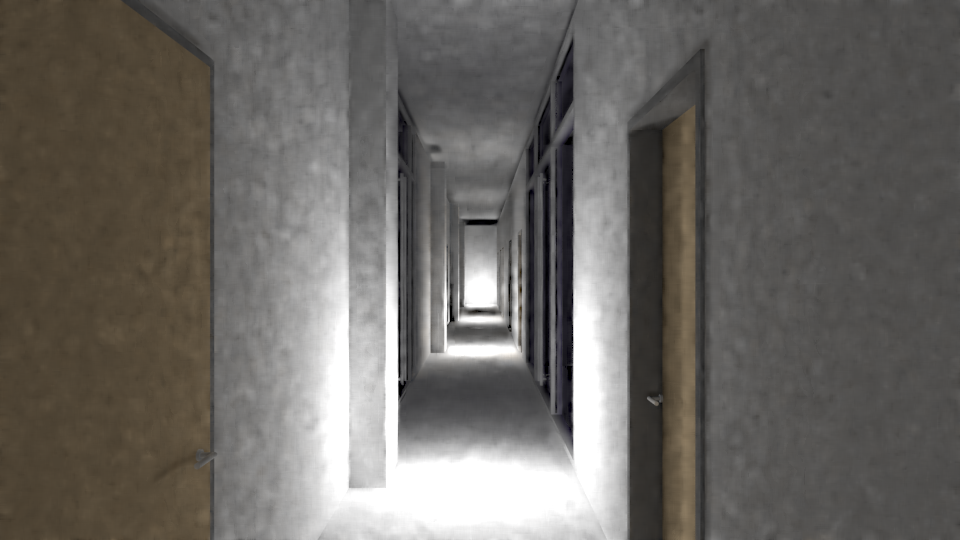
\includegraphics[width=\linewidth]{images/syn_dataset/c00708.png}
		\caption{fotorealistische \hspace{1cm} Simulation}
		\label{subfig:photorealistic}
	\end{subfigure}
	\hfill 
	\begin{subfigure}[t]{0.24\linewidth}
		\centering
		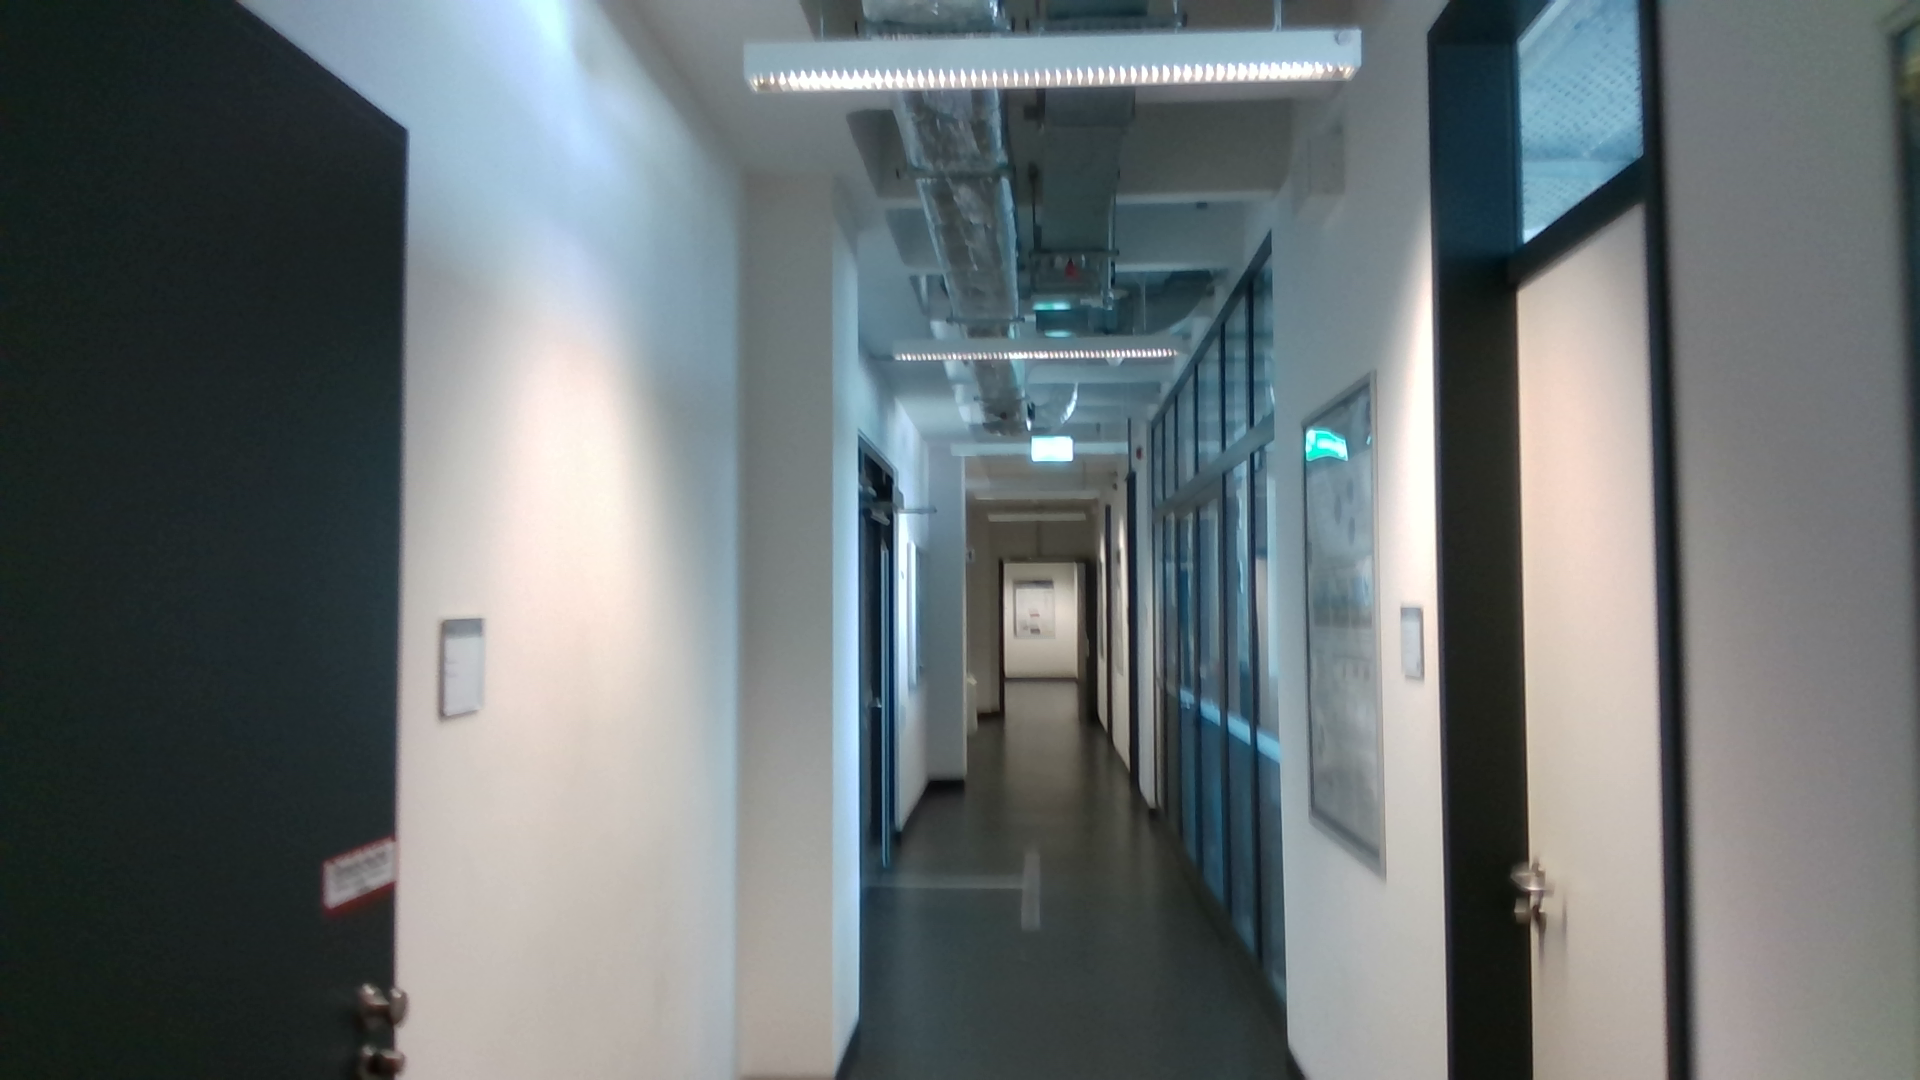
\includegraphics[width=\linewidth]{images/syn_dataset/r000305.png}
		\caption{reale Aufnahme \hspace{2cm}}
		\label{subfig:real}
	\end{subfigure}
	\hfill 
	\begin{subfigure}[t]{0.24\linewidth}
		\centering
		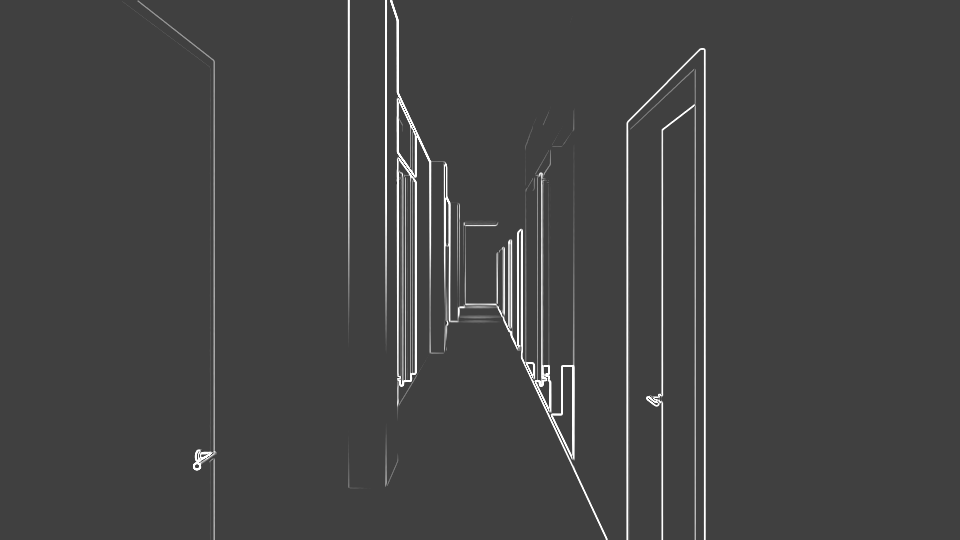
\includegraphics[width=\linewidth]{images/syn_dataset/bg00708.png}
		\caption{Gradientenbild  \hspace{1cm} von \subref{subfig:cartoonish}}
	\end{subfigure}
	\hfill
	\begin{subfigure}[t]{0.24\linewidth}
		\centering
		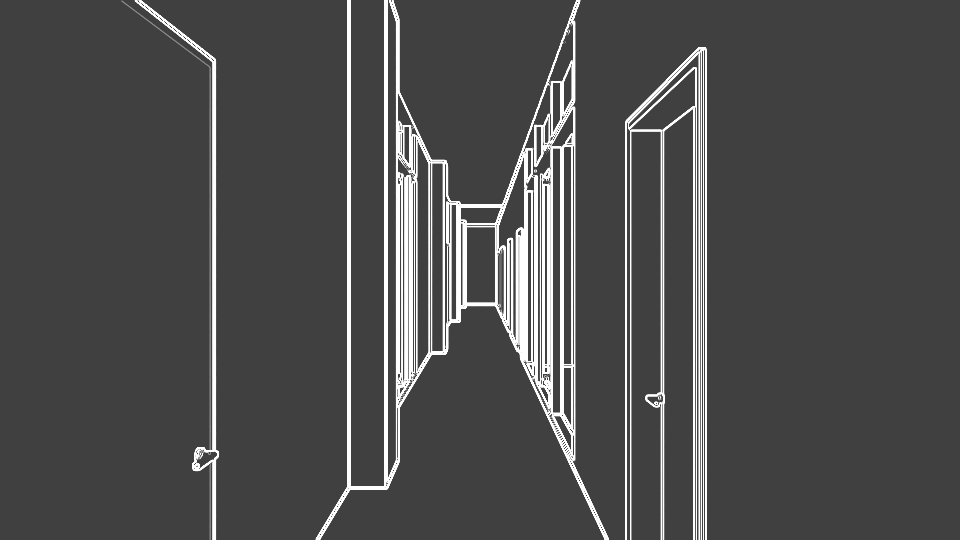
\includegraphics[width=\linewidth]{images/syn_dataset/eg00708.png}
		\caption{Gradientenbild  \hspace{1cm} von \subref{subfig:edge}}
	\end{subfigure}
	\hfill
	\begin{subfigure}[t]{0.24\linewidth}
		\centering
		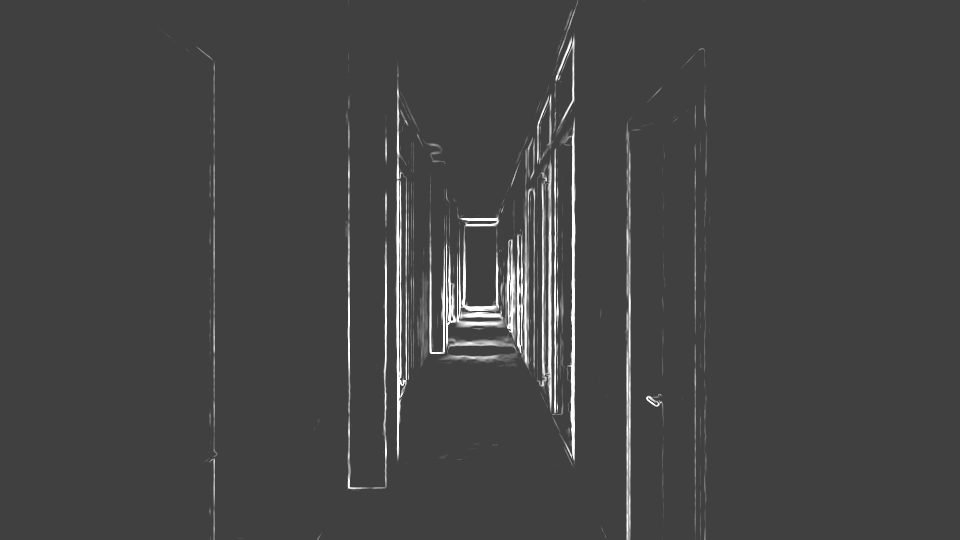
\includegraphics[width=\linewidth]{images/syn_dataset/cg00708.png}
		\caption{Gradientenbild  \hspace{1cm} von \subref{subfig:photorealistic}}
	\end{subfigure}
	\hfill
	\begin{subfigure}[t]{0.24\linewidth}
		\centering
		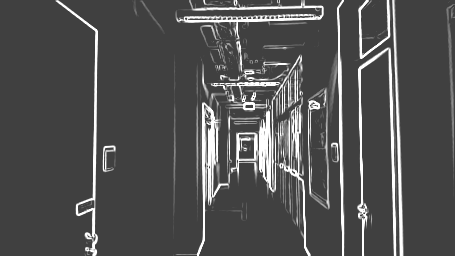
\includegraphics[width=\linewidth]{images/syn_dataset/rg000305.png}
		\caption{Gradientenbild  \hspace{1cm} von \subref{subfig:real}}
	\end{subfigure}
	\hfill
	\caption{Beispielhafte Bilder für jeden Datensatztyp und die dazu korrespondierenden Gradientenbilden. Die Daten sind aus dem \textit{IC-loop} Datensatz.}
	\label{fig:dataset_preprocess}
\end{figure}

\cleardoublepage

\subsection{Trainingsparameter}
Es wird die Caffe \cite{jiaCaffeConvolutionalArchitecture2014} Implementierung von PoseNet verwendet, die von den eigenen Autoren \citet{kendallPoseNetConvolutionalNetwork2015} veröffentlicht wurde.

Die Batchgröße beträgt 40 und die Anzahl der Trainingsepochen ist 160. Eine NVIDIA GeForce GTX 1080 Ti mit 11GB Grafikspeicher wird verwendet und ermöglicht bei einer Batchgröße von 40 drei Trainingsprozesse zeitgleich durchzuführen.

Der Hyperparameter $\beta$, der von PoseNet vorgestellten Kostenfunktion (vgl. Gleichung \ref{eq:posenet_loss}), wird für jeden realen Datensatz durch ein Grid-Search Verfahren bestimmt, indem PoseNet mit der Hälfte der realen Daten trainiert und mit der restlichen Hälfte evaluiert wird. Die Werte für den Hyperparameter werden im Abschnitt \ref{subsec:determine_beta} bestimmt und $\beta$ sind in Tabelle \ref{tab:betas} aufgelistet. Der Loss wird mit dem AdaGrad \cite{duchiAdaptiveSubgradientMethods2011} Gradientenabstiegsverfahren mit einer konstanten Lernrate von $10^{-3}$ optimiert bzw. minimiert. 

Die Trainings- sowie Evaluationsdaten werden auf eine Auflösung von $480\times270$ skaliert. Während des Trainingsprozesses werden zufällige Ausschnitte der Größe $224 \times 224$ aus dem skalierten Datensatz genommen und für die Evaluierung wird ein zentrierter Ausschnitt derselben Größe aus dem skalierten Evaluationsdatensatz verwendet. Das Durchschnittsbild der synthetischen Daten werden beim Trainieren und bei der Evaluierung von den Inputbildern subtrahiert.
Die Gewichte des Netzwerks werden mit den Gewichten eines Modells initialisiert, das auf der GoogLeNet Architektur mit dem Places Datensatz \cite{zhouLearningDeepFeatures2014} trainiert wurde. Anschließend werden die Gewichte an die Trainingsdaten angepasst. Tabelle \ref{tab:trainingparams} gibt eine Übersicht der Hyperparameter an.

\begin{table}[H]
	\centering
	\caption{Übersicht der Hyperparameter.}
	\begin{tabularx}{1.0\textwidth}{X X}
		\textbf{Hyperparameter} & \textbf{Wert}\\
		\hline
		Batchgröße & $40$\\
		\hline
		Anzahl der Epochen & $160$\\
		\hline
		$\beta$ der Kostenfunktion (vgl. Gleichung \ref{eq:posenet_loss}) &
		siehe Tabelle \ref{tab:betas} im Abschnitt \ref{subsec:determine_beta}
		\\
		\hline
		Loss-Optimierer & AdaGrad\\
		\hline
		Lernrate & $10^{-3}$\\
		\hline
		Bildskalierung & $480 \times 270$\\
		\hline
		Bildausschnitt& \makecell[tl]{
			$224 \times 244$\\
			(Training: zufällig, Evaluation: zentriert)\\
		}\\
		\hline
		Datensatznormierung & Subtraktion des Durchschnittsbildes der synthetischen Daten \\
		\hline
		Initialisierung der Gewichte & Gewichte eines mit dem Places Datensatz trainierten Modells auf GoogLeNet \\
	\end{tabularx}
	\label{tab:trainingparams}
\end{table}